\documentclass[svgnames,smaller]{beamer}\usepackage[]{graphicx}\usepackage[]{color}
% maxwidth is the original width if it is less than linewidth
% otherwise use linewidth (to make sure the graphics do not exceed the margin)
\makeatletter
\def\maxwidth{ %
  \ifdim\Gin@nat@width>\linewidth
    \linewidth
  \else
    \Gin@nat@width
  \fi
}
\makeatother

\definecolor{fgcolor}{rgb}{0.345, 0.345, 0.345}
\newcommand{\hlnum}[1]{\textcolor[rgb]{0.686,0.059,0.569}{#1}}%
\newcommand{\hlstr}[1]{\textcolor[rgb]{0.192,0.494,0.8}{#1}}%
\newcommand{\hlcom}[1]{\textcolor[rgb]{0.678,0.584,0.686}{\textit{#1}}}%
\newcommand{\hlopt}[1]{\textcolor[rgb]{0,0,0}{#1}}%
\newcommand{\hlstd}[1]{\textcolor[rgb]{0.345,0.345,0.345}{#1}}%
\newcommand{\hlkwa}[1]{\textcolor[rgb]{0.161,0.373,0.58}{\textbf{#1}}}%
\newcommand{\hlkwb}[1]{\textcolor[rgb]{0.69,0.353,0.396}{#1}}%
\newcommand{\hlkwc}[1]{\textcolor[rgb]{0.333,0.667,0.333}{#1}}%
\newcommand{\hlkwd}[1]{\textcolor[rgb]{0.737,0.353,0.396}{\textbf{#1}}}%
\let\hlipl\hlkwb

\usepackage{framed}
\makeatletter
\newenvironment{kframe}{%
 \def\at@end@of@kframe{}%
 \ifinner\ifhmode%
  \def\at@end@of@kframe{\end{minipage}}%
  \begin{minipage}{\columnwidth}%
 \fi\fi%
 \def\FrameCommand##1{\hskip\@totalleftmargin \hskip-\fboxsep
 \colorbox{shadecolor}{##1}\hskip-\fboxsep
     % There is no \\@totalrightmargin, so:
     \hskip-\linewidth \hskip-\@totalleftmargin \hskip\columnwidth}%
 \MakeFramed {\advance\hsize-\width
   \@totalleftmargin\z@ \linewidth\hsize
   \@setminipage}}%
 {\par\unskip\endMakeFramed%
 \at@end@of@kframe}
\makeatother

\definecolor{shadecolor}{rgb}{.97, .97, .97}
\definecolor{messagecolor}{rgb}{0, 0, 0}
\definecolor{warningcolor}{rgb}{1, 0, 1}
\definecolor{errorcolor}{rgb}{1, 0, 0}
\newenvironment{knitrout}{}{} % an empty environment to be redefined in TeX

\usepackage{alltt}
\usetheme[progressbar=none, numbering=fraction]{metropolis}

% define colors
\setbeamercolor{frametitle}{bg=SteelBlue}
\setbeamercolor{progress bar}{fg=SteelBlue}
\setbeamercolor{background canvas}{bg=White}

\newcounter{saveenumerate}
\makeatletter
\newcommand{\enumeratext}[1]{%
\setcounter{saveenumerate}{\value{enum\romannumeral\the\@enumdepth}}
\end{enumerate}
#1
\begin{enumerate}
\setcounter{enum\romannumeral\the\@enumdepth}{\value{saveenumerate}}%
}
\makeatother

\setlength{\leftmargini}{2em}

% \setbeamertemplate{itemize items}[default]
% \setbeamertemplate{enumerate items}[default]

\usepackage{amsmath}
\usepackage{amsfonts}
\usepackage{bm}
\usepackage{hyperref}
\hypersetup{
    colorlinks=true,
    linkcolor=magenta,
    filecolor=magenta,      
    urlcolor=magenta,
}
\setbeamertemplate{footline}{}
\setbeamertemplate{logo}{%
    \usebeamercolor[fg]{footline}%
    \usebeamerfont{page number in head/foot}%
  \usebeamertemplate*{frame numbering}\hspace{6pt}%
}

\usepackage{booktabs}
\usepackage{multirow}
\usepackage{pgf, tikz}
\usepackage{tkz-tab}
\usetikzlibrary{shapes,decorations,arrows,calc,arrows.meta,fit,positioning}
\usetikzlibrary{arrows,shapes.arrows,shapes.geometric,shapes.multipart,
decorations.pathmorphing,positioning}
\tikzstyle{arrow}=[->, >=stealth]
\tikzset{
    -Latex,auto,node distance =1 cm and 1 cm,semithick,
    state/.style ={ellipse, draw, minimum width = 0.7 cm},
    cond/.style ={rectangle, draw, minimum width = 0.7 cm},
    point/.style = {circle, draw, inner sep=0.04cm,fill,node contents={}},
    bidirected/.style={Latex-Latex,dashed},
    el/.style = {inner sep=2pt, align=left, sloped}
}
\usepackage{subcaption}
\usepackage{caption}

\usepackage{tcolorbox}
\tcbuselibrary{listings,breakable, skins}
\newcommand\dummy[1]{#1}
\let\Begin\begin
\let\End\end
\newenvironment{tcbmagenta}[1]
    {\dummy{\Begin{tcolorbox}[enhanced, breakable=true, title = #1, colback=white, colframe=magenta!75]}
    }
    {
    \End{tcolorbox}
    }

% magenta bold command
\newcommand{\bmagenta}[1]{\textcolor{magenta}{\textbf{#1}}}

% mathhbb E
\newcommand{\E}{\mathbb{E}}

\newcommand{\indep}{\perp \!\!\! \perp}
\IfFileExists{upquote.sty}{\usepackage{upquote}}{}
\begin{document}




%%%%%%%%%%%%%%%%%%%%
%% TITLE FRAME
%%%%%%%%%%%%%%%%%%%%%%%%%%%%%%%%%%%%%%%%%%%%%%%%%%%%%%%%%%%%%%%%%%%%%%%%%%%%%%%%%%%%%% TITLE
{
\setbeamercolor{background canvas}{bg=SteelBlue!30}
\begin{frame}
\begin{center}
\vspace{0cm}\large \textcolor{SteelBlue!95}{\textbf{Getting started with R}} \\

{\color{Snow}\hrulefill}

\textcolor{SteelBlue!95}{Matt Lee (mlee8@g.harvard.edu), PHS Launch 2022}
\end{center}
\end{frame}
}

\small

%%%%%%%%%%%%%%%%%%%%%%%%%%%%%%%%%%%%%%%%%%%%%%%%%%%%%%%%%%
%%
%%  What is R
%%
%%%%%%%%%%%%%%%%%%%%%%%%%%%%%%%%%%%%%%%%%%%%%%%%%%%%%%%%%%

\begin{frame}{What is R?}

\begin{itemize}
    \item R is an open-source \textbf{interpreted} programming language: when you install R, you install an \textit{interpreter} that translates your R code into computer code (sometimes called ``machine'' code), which is what actually gets run
    \item This is in contrast to \textbf{compiled} languages (e.g. C or C++), where the programmer writes code that is directly converted into machine code
    \item Several advantages of interpreted languages: much more user friendly, easily read, consistent across operating systems
    \item Some disadvantages: often slower, and less control over system hardware$^*$
\end{itemize}

\vspace{1em}

\bmagenta{Action step:} Install R (https://cloud.r-project.org/) 

\end{frame}


%%%%%%%%%%%%%%%%%%%%%%%%%%%%%%%%%%%%%%%%%%%%%%%%%%%%%%%%%%
%%
%%  R studio
%%
%%%%%%%%%%%%%%%%%%%%%%%%%%%%%%%%%%%%%%%%%%%%%%%%%%%%%%%%%%

\begin{frame}{R Studio: Integrated Development Environments (IDEs)}

\begin{itemize}
    \item We can interact with R directly via a command line (e.g. Terminal)
    \begin{figure}[tb]
    \centering
    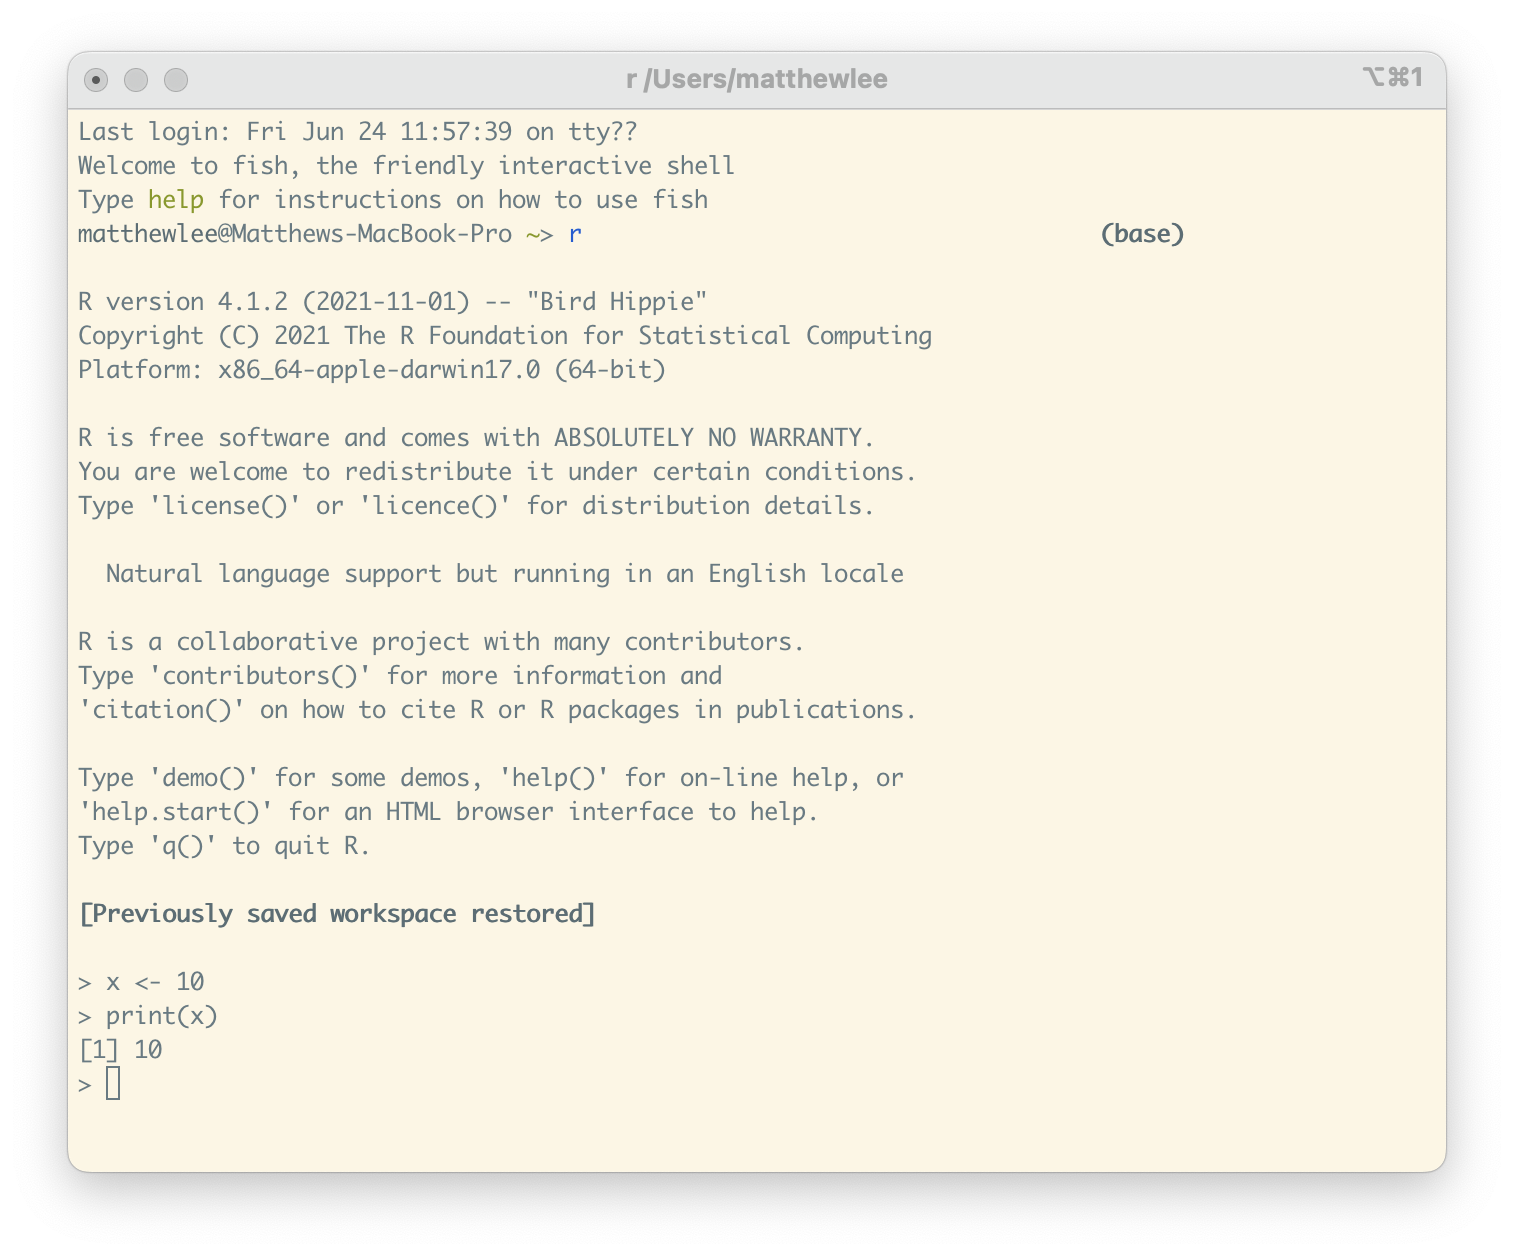
\includegraphics[width = .35\textwidth]{R-terminal.png}
    \end{figure}
    \item But this is not very pretty or reproducible! A population alternative is to use an IDE, such as R Studio, which is a program that adds a whole lot of convenience to writing and running R code
    \item IDEs are not the language themselves, they provide a way to interact with the language installed on your computer in a friendly way
\end{itemize}

\bmagenta{Action step:} Install R Studio (https://www.rstudio.com/products/rstudio/download/) 


\end{frame}


%%%%%%%%%%%%%%%%%%%%%%%%%%%%%%%%%%%%%%%%%%%%%%%%%%%%%%%%%%
%%
%%  Working in R Studio
%%
%%%%%%%%%%%%%%%%%%%%%%%%%%%%%%%%%%%%%%%%%%%%%%%%%%%%%%%%%%

\begin{frame}{Working in R Studio}

Key R Studio panes:
\begin{itemize}
    \item Console: Runs R code, either interactively or via an R script
    \item Terminal: Convenient terminal application (primarily useful for version control programs like git/GitHub)
    \item Environment: Objects you've saved to your \textbf{working R environment}
    \item Files: File navigator, useful if you need to figure out where data/R scripts are located
    \item Plots: Plots generated will populate in this pane -- you can also export plots you create using the ``Export'' button
\end{itemize}

\end{frame}


%%%%%%%%%%%%%%%%%%%%%%%%%%%%%%%%%%%%%%%%%%%%%%%%%%%%%%%%%%
%%
%%  R scripts
%%
%%%%%%%%%%%%%%%%%%%%%%%%%%%%%%%%%%%%%%%%%%%%%%%%%%%%%%%%%%

\begin{frame}{R Scripting}

Use of an \textbf{R script} helps keep your code neat and reproducible
\begin{itemize}
    \item In R Studio: File $\rightarrow$ New File $\rightarrow$ R Script
    \item This is simply a text file with the extension ``.R'' that will hold all of the R commands we want to run
    \item Similar to other languages, ``\#'' is reserved for comments
\end{itemize}

There are 5 main \textbf{data types} in R:
\begin{itemize}
    \item Character (e.g. \texttt{"hello world"})
    \item Numeric (e.g. \texttt{3.14159265})
    \item Integer (e.g. \texttt{5L})
    \item Logical (\texttt{TRUE}, \texttt{FALSE})
    \item Complex (\texttt{1i})
\end{itemize}

\end{frame}

%%%%%%%%%%%%%%%%%%%%%%%%%%%%%%%%%%%%%%%%%%%%%%%%%%%%%%%%%%
%%
%%  R scripts
%%
%%%%%%%%%%%%%%%%%%%%%%%%%%%%%%%%%%%%%%%%%%%%%%%%%%%%%%%%%%

\begin{frame}{R Scripting}

R also has various \texttt{data structures}, but the main ones are:
\begin{itemize}
    \item Vectors: a collection of elements of one data type
    \item Lists: a collection of objects of arbitrary types (e.g. the first element could be a vector, the second element could be a matrix, the third element could be a data frame)
    \item Matrices: a vector (so much be one data type only), with dimensions defined
    \item Data frames: structure that most resembles a data set, each variable is a single data type
    \item Factors: a numeric vector that has a label attribute
\end{itemize}

\end{frame}



%%%%%%%%%%%%%%%%%%%%%%%%%%%%%%%%%%%%%%%%%%%%%%%%%%%%%%%%%%
%%
%%  Open questions/work
%%
%%%%%%%%%%%%%%%%%%%%%%%%%%%%%%%%%%%%%%%%%%%%%%%%%%%%%%%%%%

\begin{frame}{Troubleshooting/Q\&A}



\end{frame}





\end{document}
